\documentclass{article}


% if you need to pass options to natbib, use, e.g.:
%     \PassOptionsToPackage{numbers, compress}{natbib}
% before loading neurips_2022


% ready for submission
\usepackage{amsmath}
\usepackage[preprint]{neurips_2022}
\bibliographystyle{ieeetr}      % TODO, throwing an error for some reason


% to compile a preprint version, e.g., for submission to arXiv, add add the
% [preprint] option:
%     \usepackage[preprint]{neurips_2022}


% to compile a camera-ready version, add the [final] option, e.g.:
%     \usepackage[final]{neurips_2022}


% to avoid loading the natbib package, add option nonatbib:
%    \usepackage[nonatbib]{neurips_2022}

\usepackage[utf8]{inputenc} % allow utf-8 input
\usepackage[T1]{fontenc}    % use 8-bit T1 fonts
\usepackage{hyperref}       % hyperlinks
\usepackage{graphicx}
\usepackage{float}
\usepackage{url}            % simple URL typesetting
\usepackage{booktabs}       % professional-quality tables
\usepackage{amsfonts}       % blackboard math symbols
\usepackage{nicefrac}       % compact symbols for 1/2, etc.
\usepackage{microtype}      % microtypography
\usepackage{xcolor}
\usepackage{amssymb}
\usepackage{tikz}         % colors
\usetikzlibrary{shapes.multipart}
\usetikzlibrary{positioning, arrows.meta}
\newcommand{\new}[1]{{\color{red} #1}}

\title{ELSAN: Efficient Ensemble Forecasting of Chaotic Systems}


\author{%
  Manu, Bhat \\
  Department of Computer Science\\
  UC San Diego\
  La Jolla, CA 92093 \\
  \texttt{mbhat@ucsd.edu} \\
}


\begin{document}

\maketitle


\begin{abstract}
    Although traditional approaches to deep learning in chaotic systems focus on generating the most likely option given an initial state, this may be misleading as one sample simply does not contain enough information to encompass the entire system. On the other hand, an ensemble forecast composing of hundreds of simulations with varied initial conditions helps provide a more nuanced image, but is computationally intensive. We present an alternative option, Ensemble Linear Sum Assignment Network (ELSAN), that outputs many possible options for a final state without full recomputation. In particular, instead of producing a single frame in time, ELSAN produces an encoding of the final distribution, which can then be queried quickly to produce many possible final states. We use the case study of turbulent flow to prove out the model and provide a comparison with traditional deep learning approaches and numerical simulations. Our work is publicly available on \href{https://github.com/enigmurl/tf-net-confidence-domain}{GitHub}.
\end{abstract}

\section{Introduction}

\paragraph{Problem Definition.}

In the context of chaotic systems, a small change to the input leads to large, unpredictable changes to the output. What's worse is that in the real world, measurements of the initial state are bound to have some level of imprecision to them. This leads to the following problem: because we have an imperfect measurement and that error grows exponentially across prediction steps, it is fundamentally impossible to make a single, accurate prediction far into the future. One partial remedy especially prevalent in metereology is to generate an ensemble—or collection—of samples. \cite{TyphoonEnsemblePredictionSystemDevelopedattheJapanMeteorologicalAgency}. From here, one can make probabilistic statements about the final outcome. However, this is typically done using a Monte-Carlo simulation. We present a more efficient method of ensemble forecasts that does not require a full re-simulation for each member.

For the purpose of the paper, we specifically focus on the problem of turbulent fluid simulations, but keep in mind that the techniques we introduce aim to be environment-agnostic.
\paragraph{Problem Significance.}
Our work can theoretically can be applied to many real-world scenarios. Of course, turbulent flow and related phenomena are of extreme relevance. One could make ensemble forecasts of hurricanes and other weather phenomena efficiently. On a smaller scale, coast guard and search-and-rescue teams could simulate thousands of possible ending locations given a known initial position for a person lost at sea. Finally, we note that ensemble forecasting is relevant outside fluid dynamics and is pertinent to practically any chaotic system. One can simulate the three-body problem or the origins of the solar system.
\paragraph{Technical Challenges.}
One of the harder parts of tackling the problem is that we not only need to output a varied amount of final states, but that probability distribution of final states should match the ground truth. This is a challenge because deep learning models typically focus on a single input and output, rather than a full distribution. We tackle this challenge by taking advantage of the linear sum assignment problem to measure distances between distributions.

Related to the first issue, the majority of datasets are sparse in the sense that for a given input in dataset, most other datapoints will have their inputs be far away. This is good for most models since it gives a diverse training set. However, it is not necessarily great for our situation since we would prefer a dataset which is dense and has many inputs that are close together. For this reason, we create our own simulated dataset.

Perhaps the most difficult part is the fact that it's hard to even predict a mean, let alone the entire distribution. This often leads to mode collapse, as the model concentrates the distribution to the point closest to the true distribution. For this paper, our goal is that even if we cannot make the distributions overlap, we will try to make their shapes as similar as possible. This may not always be ideal in all circumstances, but is nevertheless how we proceed. An illustration is provided in Figure~\ref{separate_distributions}.

\begin{figure}
    \centering
    \caption{
        In chaotic systems, it's hard to get a single prediction, let alone an entire ensemble. This typically means that any given prediction is far away from the ground truth, which consequently leads some networks (left) to mode collapse. Our work (right) tries to mirror the shape of the distribution, even if the means are impossible to perfectly match.
    }
    \label{separate_distributions}
    \fbox{ \includegraphics[width=15em]{mode_collapse} }
    \fbox{ \includegraphics[width=15em]{mirror_distribution} }
\end{figure}

\paragraph{State of the Art.}
Due to the complex nature of probability distributions and the fact that they are generally intractable, typical approaches to problems of this nature tend to either be likelihood-based or generative models. In particular, Variational Auto Encoders and Generative Adversarial Networks are extremely powerful in this space. We will compare our results to these models towards the end of the paper \cite{goodfellow2014generative, kingma2022autoencoding, doersch2021tutorial}.

\paragraph{Contributions.}
\begin{itemize}
    \item Contribution 1: We propose using square root decomposition in the context of temporal networks to speed up training and inference.
    \item Contribution 2: We introduce a model and training method utilizing the linear sum assignment problem.
\end{itemize}

\section{Related Work}

\paragraph{Ensemble Forecasting} Ensemble forecasting, like that done in TEPS \cite{TyphoonEnsemblePredictionSystemDevelopedattheJapanMeteorologicalAgency}. is generally performed via a Monte-Carlo simulation. Essentially, the initial conditions are slightly perturbed and a fully deterministic simulation is run using these various conditions. Some variations may introduce noise past the initial frame, but the basic idea remains. In the TEPS paper, the purpose of the ensemble is to actually use an ensemble mean instead of the probability distribution. Nevertheless, it provides a useful reference point.

\paragraph{Turbulent Flow Forecasting} Turbulent Flow forecasting is a tough problem by itself and has many approaches to solve it, including Large Eddy Simulations (LES) and Reynolds-averaged Navier Sokes (RANS). Turbulent Flow Net (TF-net) \cite{Wang2020TF} combines these techniques into a single network. Its other innovations include using temporal and spatial filtering, leading to an extremely performant model.

\section{Methodology}

\paragraph{Problem Setting.}
Formally, our general problem is given an initial state $s_0$ with an implicit amount of imprecision and $F(t, s_0)$ which is a function of time given initial state, we would like to compute the probability distribution $P$ such that $P(t,s)$ = the likelihood that $F(t,s_0) = s$.

In the context of our turbulent flow, this means that given a measurement of velocity field to a certain amount of significant figures, predict the likelihood of any final velocity field $t$ frames into the future. In practice, $P$ is encoded implicitly by the model, and we only look to sample from the distribution.

\paragraph{Idea Summary.}
The high level idea of our work is to output a latent space encoding of the entire distribution of final output states given an input state. In particular, we compute the mean of the latent space of the result explicitly. Implicitly, we also encode the probability distribution of the errors. For clarity, suppose we want to generate $128$ predictions. To do this, we will first query the mean latent space vector, $\hat{\mu} \in Z$ where $Z$ denotes the entirety of the latent space. Then, we will query $128$ errors from the implicit distribution, say $\hat{\delta} \in Z^{128}$. To compute the $i$th prediction, we calculate $\hat{\mu} + \hat{\delta}_{i}$, and then use a final clipping layer to convert this latent space encoding into a sample. This is repeated $128$ times. Thus, to compute these predictions, we do not need to rerun the entire model every time, only the final clipping layer (which is relatively inexpensive).

\paragraph{Linear Sum Assignment.}
Before introducing the full description of the model, we would like to familiarize the reader with the linear sum assignment (LSA) problem \cite{linearsumassignment}. LSA is sometimes also referred to as minimal perfect bipartite matching, or just matching. Regardless, suppose we are given a matrix $A \in \mathbb{R}^{N \times N}$. Then, LSA gives us a permutation $\sigma$ of the integers $1 \ldots N$ that minimizes the following constraint over all such permutations.
\[
    \min_{\sigma \in S_{n}} \sum_{i = 1}^{n} A_{i, \sigma_i}
\]
For motivation on why this is useful to our problem, consider if we are given two sets $P, Q$ of $N$ points in $\mathbb{R}^2$ and $A_i,j$ is defined to be the Euclidean distance between $P_i$ and $Q_j$. In such a case, the value of LSA is a measure of how dissimilar the two sets are. To formalize this, we show how LSA can be taken to be a metric. Suppose we are given a metric space $(Q, d)$ where $d: Q \times Q \to \mathbb{R}$ is the distance function for the metric. We define the LSA metric space over $(Q,d)$ as $(Q^{N}, lsa)$ for some arbitrary integer $N$, and $lsa$ is defined to be the following. Note that in our definition, we consider $X = Y$ if $X$ is a permutation of $Y$.
\[
    lsa(X,Y) = \min_{\sigma \in S_{n}} \sum_{i = 1}^{J} A_{i, \sigma_i} \text{ where } A_{i, j} = d(X_i, Y_{j})
\]
We claim this forms a metric space. First note that since $d$ is a metric, all values of $A$ are non-negative and any permutation results in a non-negative total cost. Then, $X = Y \to lsa(X,Y) = 0$ since the value $0$ is induced by whatever permutation sends $X$ to $Y$. For positivity, assume that $lsa(X, Y) = 0$. Then, there exists a $\sigma \in S_n$ such that $\sum_{i = 1}^{N}d(X_i, Y_{\sigma_{i}}) = 0$, which implies that $d(X_i, Y_{\sigma_{i}}) = 0$ for all $i$, which tells us that $X$ is a permutation of $Y$. Thus, $lsa$ only gives zero values for equal inputs and otherwise is positive. Symmetry follows from the fact that any assignment in $A$ is an assignment in $A^{T}$. For the triangle inequality, assume we are given $X, Y, Z \in Q^{N}$. Then, suppose we are given the permutation $\sigma$ that minimizes $lsa(X, Y)$ and similarly the permutation $\tau$ for $lsa(Y, Z)$. Now, consider the permutation $\rho = \tau\sigma$. Then,
\begin{align*}
    lsa(X, Z) & \le \\
    \sum_{i = 0}^{N}d(X_{i}, Z_{\rho_{i}}) & \le \\
    \sum_{i = 0}^{N}d(X_{i}, Y_{\sigma_{i}}) + d(Y_{\sigma_{i}}Z_{\rho_{i}}) & = \\
    \sum_{i = 0}^{N}d(X_{i}, Y_{\sigma_{i}}) + \sum_{i = 0}^{N} d(Y_{\sigma_{i}}Z_{\tau_{\sigma_{i}}}) & = \\
    lsa(X, Y) + lsa(Y, Z)
\end{align*}

Therefore, $lsa(X, Z) \le lsa(X, Y) + lsa(Y, Z)$ and $(Q^N, lsa)$ forms a metric space. $lsa$ thus provides a simple, computationally efficient way to compare distributions \cite{linearsumassignment}.
\paragraph{Description.}
We now introduce our model. Assume that we are given the last $i$ time steps of a fluid's velocity field, and want to create $s$ predictions $t$ time steps into the future. With this, the base model first encodes this into what is called the pruning vector $v$. Then, a transition model is iteratively run on the pruning vector $t$ times. From the updated pruning vector and $s$, $\hat{\mu} \in Z$ and $\hat{\delta} \in Z^{s}$ are calculated using a clipping layer. Note that $\hat{\mu} + \hat{\delta}_i \in Z$, the latent space. Finally, a decoder converts each $\hat{\mu} + \hat{\delta}_i$ to a pixel space representation. A diagram is provided in Figure~\ref{model}.

Crucially, for training, a single seed is given and ELSAN returns $\hat{\mu}$ and $\hat{\delta}$. An encoder converts the ground truth into the latent space, where we can find $\mu$ and $\delta$, the true mean and true delta. Then, the loss function is the mean absolute difference between $\mu$ and $\hat{\mu}$ plus the linear sum assignment between $\delta$ and $\hat{\delta}$. The submetric for LSA is taken to be RMSE. This is optimized via stochastic gradient descent. In our work, we use $L = 128$. The encoder and decoder pair is trained separately, which is detailed later.

To reduce memory usage, and improve training and inference speed, we introduce square root decomposition. In particular, we have two transition models. One that advances the pruning vector $K$ steps and one that advances a single time step. If we know that we will never need to predict more than $T$ timesteps into the future, it is generally optimal to set $K = \lceil\sqrt {T}\rceil$, ensuring that no more than $O\left(\sqrt{t}\right)$ transitions are applied for a single prediction querying time $t$. This also has the added benefit of reducing exploding or diminishing gradients.
\paragraph{Implementation.}
We implement the model through PyTorch using the TF-net \cite{Wang2020TF} codebase as a starting point for the base model. In addition, hyperparameters are more or less adapted from the original paper, with minor modifications to adapt to the new model. The other models are implemented using standard U-net architectures.

A crucial step during implementation is the separation of the encoder-decoder pair from the main network. Without this modification, we found the decoder would cheat by squishing the latent space to a very tiny ball so that the $lsa$ function will always be small. As such, it is recommended to either train the decoder in parallel, or use a fixed decoder. We also train the networks producing $\mu$ and $\delta$ using different optimizers, but this step is not as significant.
    
Note that computing a backward pass naively, even with square root decomposition, may lead to memory constraints. However, a forward pass is typically not a problem. Therefore, the optimal permutation from $lsa$ is calculated in the forward pass as normal and saved. Then, in the backward pass, the permutation is partitioned into a set of sub-arrays, each of small length. A backward pass is computed on each subarray, reducing memory pressure.

A final important implementation detail which we found to boost performance is the introduction of a warm-up phase. In essence, for the first few epochs, we only train 1 frame in advance. Then, the limit is raised to two. Later, it is raised to three and the process continues all the way to the limit of the dataset.

\begin{figure}
    \centering
    \caption{ELSAN Network. Layers that are used in the inference main run are shown in blue. Layers that are used in the main network solely for training are black and dotted. Layers that are just used for the autoencoder training are shown in red. For the autoencoder network, the loss is the RMSE between the input and the output. For the main network, the loss is the $lsa$ between the clipping differences and the ground truth clipping differences summed with the absolute differences between the ground truth mean and the predicted mean in the latent space. }
    \label{model}

    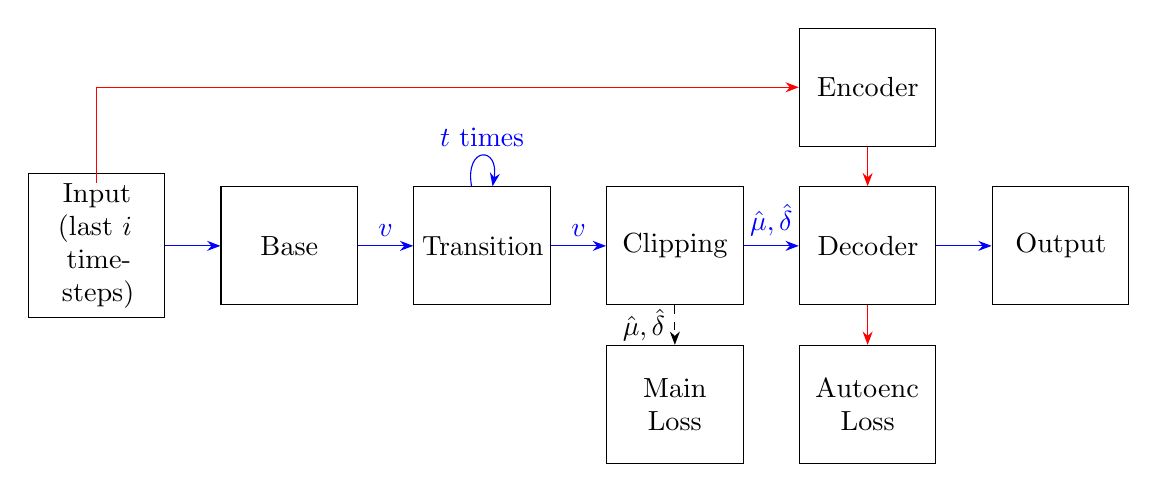
\begin{tikzpicture}[
        block/.style={rectangle, draw, text width=1.5cm, align=center, minimum height=1.5cm},
        arrow/.style={-Stealth}
    ]
        \node[block] (input) {Input (last $i$ time-steps)};

        \node[block, right=0.7cm of input] (base) {Base};

        \node[block, right=0.7cm of base] (transition) {Transition};

        \node[block, right=0.7cm of transition] (clipping) {Clipping};
        \node[below=0.5cm of clipping, block] (mainloss) { Main Loss};

        \node[block, right=0.7cm of clipping] (decoder) {Decoder};
        \node[above=0.5cm of decoder, block] (encoder) {Encoder};
        \node[below=0.5cm of decoder, block] (loss) { Autoenc Loss};
        \node[block, right=0.7cm of decoder] (output) {Output};

        \draw[arrow, red] (input) -- ++(0,0.8) |- (encoder);
        \draw[arrow, red] (encoder) -- (decoder);
        \draw[arrow, red] (decoder) -- (loss);
        \draw[arrow, blue] (input) -- (base);
        \draw[arrow, blue] (base) -- node[above] {$v$} (transition);
        \draw[arrow, blue] (transition) -- node[above] {$v$} (clipping);
        \draw[arrow, blue] (clipping) -- node[above] {$\hat{\mu}, \hat{\delta}$} (decoder);
        \draw[arrow, blue] (decoder) -- (output);
        \draw[arrow, blue] (transition) to[out=100,in=80, looseness=5] node[above] {$t$ times} (transition);
        \draw[arrow, black, dashed] (clipping) -- node[left] {$\hat{\mu}, \hat{\delta}$} (mainloss);
%        \draw[arrow, black, dashed] (encoder) -- (mainloss);
    \end{tikzpicture}

\end{figure}

\section{Experiments}
\paragraph{Datasets and Tools.}
Our dataset was created using the fluidsim python package \cite{fluiddyn, fluidfft, fluidsim}. We use a reynolds number of $3 \times 10^6$. $128$ seed inputs were simulated, with each one producing a $128$ member ensemble. Each member contains $32$ timesteps, each being a tensor with shape 63x63x2. A relatively large time step of 1.2s/frame was taken to induce purposeful chaos. This was done by simulating $6$ frames of $0.2$s, and then only keeping the last one. The dataset was created on an Apple M1 Pro and took around $48$ hours for the creation and post processing. We trained the machine learning model on a GTX 1080ti and RTX 2080ti, with a total training time of approximately 6 hours and 200 epochs.
\paragraph{Baselines.}
We compare ELSAN with a Conditional Generative Adversarial Network (CGAN) and a Conditional Variational Autoencoder (CVAE)\cite{doersch2021tutorial, kingma2022autoencoding, goodfellow2014generative}. All models have similarities in their architecture in the sense that the only differences between the models are those that are strictly necessary for the different types of networks. Also, we note that all models take inspiration from the work of TF-Net \cite{Wang2020TF}.

\paragraph{Quantitative Results.}
We plot the LSA metric for ELSAN, CVAE, and CGAN against the ground truth for all timesteps $t$. Do note that this is the LSA on pixel space, not latent space as is done in ELSAN. We also plot the standard deviation between samples, again across time. Finally, a comparison of model parameters is given in Table~\ref{modelparams}.

\begin{figure}
    \centering
    \caption{Relevant statistics for ELSAN, CGAN, and CVAE. Epoch time is taken on a GTX 1080 ti.}
    \label{modelparams}
    \begin{tabular}{|c|c|c|}
        \hline
        Model & Parameters (millions) & Epoch Time (minutes) \\
        \hline
        ELSAN (ours) & 54 & 2.8\\
        \hline
        CGAN & 34 & 0.4 \\
        \hline
        CVAE & 34 & 0.5 \\
        \hline
    \end{tabular}
\end{figure}

\begin{figure}
    \centering
    \begin{minipage}{0.4 \textwidth}
        \centering
        \includegraphics[width=6cm]{std}
        \caption{For every timestamp and model (including the ground truth), we compute the standard deviation of every single pixel across the predicted distribution, and then average the results.}
        \label{standard_deviation}
    \end{minipage}
    \hspace{1cm}
    \begin{minipage}{0.4 \textwidth}
        \centering
        \includegraphics[width=6cm]{lsa}
        \caption{For every timestamp and model, we compute the LSA (over RMSE) between the ground truth and the predicted output distribution in pixel space.}
        \label{output_lsa}
    \end{minipage}
\end{figure}

\paragraph{Qualitative Results.}
We present the output of the ground truth, ELSAN, CVAE, and CGAN at various timestamps. We show samples of the raw pixel space outputs, as well as the differences between each ensemble member and the mean to highlight the spread of the distribution.

\begin{figure}
    \centering
    \includegraphics[width=\textwidth]{t=5}
    \caption{Output of various models at t = 5. Each row presents $4$ samples from a single model (or the ground truth) given the same input seed. This is presented as 4 pairs of two images. The left of each pair represents the x component of the predicted velocity vector, and the right represents the y component. }
    \label{t=5}
\end{figure}

\begin{figure}
    \centering
    \includegraphics[width=\textwidth]{t=10}
    \caption{Output of various models at t = 10.}
    \label{t=10}
\end{figure}

\begin{figure}
    \centering
    \includegraphics[width=\textwidth]{t=20}
    \caption{Output of various models at t = 20.}
    \label{t=20}
\end{figure}

\begin{figure}
    \centering
    \includegraphics[width=\textwidth]{t=30}
    \caption{Output of various models at t = 30.}
    \label{t=30}
\end{figure}

\begin{figure}
    \centering
    \includegraphics[width=\textwidth]{t=30diff}
    \caption{For each model and ensemble member, we compute the pixel space prediction minus the ensemble mean and plot the results for t = 30. Results are magnified by a factor of 10, but otherwise use the same color scale as before.}
    \label{t=30diff}
\end{figure}

\paragraph{Problems.}
Even though ELSAN does produce a larger spread of results than a CGAN or CVAE, the spread is somewhat inorganic and does not qualitatively match the target distribution. We hypothesize this may happen because the number of samples fed into a given training run is too small. Also, it might be the fact that the actual ensemble loss step is performed so far away from the final clipping layer that even a tiny error accumulates. While this is the main problem, other problems include a generally non-realistic and noisy image for any given sample. This is likely due to similar issues, and possibly due to the complexity of having so many optimizers, thereby exponentiation the error once again.

\section{Conclusion and Discussion}

We introduce a general framework for efficient ensemble forecasting through the idea of confidence domains. Many chaotic systems are best analyzed in a probabilistic manner, which ELSAN attempts to do. We also introduce other ideas that may be applicable in the general scope of spatiotemporal models, such as the application of square-root decomposition. Moreover, we empasize the potential that the linear sum assignment has as an auxiliary loss function and hope to see continued progress in this regard.

\bibliography{references}

%%%%%%%%%%%%%%%%%%%%%%%%%%%%%%%%%%%%%%%%%%%%%%%%%%%%%%%%%%%%
\section*{Checklist}


%%% BEGIN INSTRUCTIONS %%%
The checklist follows the references.  Please
read the checklist guidelines carefully for information on how to answer these
questions.  For each question, change the default \answerTODO{} to \answerYes{},
\answerNo{}, or \answerNA{}.  You are strongly encouraged to include a {\bf
justification to your answer}, either by referencing the appropriate section of
your paper or providing a brief inline description.  For example:
\begin{itemize}
  \item Did you include the license to the code and datasets? \answerYes{See Section~\ref{gen_inst}.}
  \item Did you include the license to the code and datasets? \answerNo{The code and the data are proprietary.}
  \item Did you include the license to the code and datasets? \answerNA{}
\end{itemize}
Please do not modify the questions and only use the provided macros for your
answers.  Note that the Checklist section does not count towards the page
limit.  In your paper, please delete this instructions block and only keep the
Checklist section heading above along with the questions/answers below.
%%% END INSTRUCTIONS %%%


\begin{enumerate}


\item For all authors...
\begin{enumerate}
  \item Do the main claims made in the abstract and introduction accurately reflect the paper's contributions and scope?
    \answerTODO{}
  \item Did you describe the limitations of your work?
    \answerTODO{}
  \item Did you discuss any potential negative societal impacts of your work?
    \answerTODO{}
  \item Have you read the ethics review guidelines and ensured that your paper conforms to them?
    \answerTODO{}
\end{enumerate}


\item If you are including theoretical results...
\begin{enumerate}
  \item Did you state the full set of assumptions of all theoretical results?
    \answerTODO{}
        \item Did you include complete proofs of all theoretical results?
    \answerTODO{}
\end{enumerate}


\item If you ran experiments...
\begin{enumerate}
  \item Did you include the code, data, and instructions needed to reproduce the main experimental results (either in the supplemental material or as a URL)?
    \answerTODO{}
  \item Did you specify all the training details (e.g., data splits, hyperparameters, how they were chosen)?
    \answerTODO{}
        \item Did you report error bars (e.g., with respect to the random seed after running experiments multiple times)?
    \answerTODO{}
        \item Did you include the total amount of compute and the type of resources used (e.g., type of GPUs, internal cluster, or cloud provider)?
    \answerTODO{}
\end{enumerate}


\item If you are using existing assets (e.g., code, data, models) or curating/releasing new assets...
\begin{enumerate}
  \item If your work uses existing assets, did you cite the creators?
    \answerTODO{}
  \item Did you mention the license of the assets?
    \answerTODO{}
  \item Did you include any new assets either in the supplemental material or as a URL?
    \answerTODO{}
  \item Did you discuss whether and how consent was obtained from people whose data you're using/curating?
    \answerTODO{}
  \item Did you discuss whether the data you are using/curating contains personally identifiable information or offensive content?
    \answerTODO{}
\end{enumerate}


\item If you used crowdsourcing or conducted research with human subjects...
\begin{enumerate}
  \item Did you include the full text of instructions given to participants and screenshots, if applicable?
    \answerTODO{}
  \item Did you describe any potential participant risks, with links to Institutional Review Board (IRB) approvals, if applicable?
    \answerTODO{}
  \item Did you include the estimated hourly wage paid to participants and the total amount spent on participant compensation?
    \answerTODO{}
\end{enumerate}

\section{Questions}
\begin{enumerate}
    \item I used a paper for learning a subject (VAE), do I need to cite them?
    \item GAN was a bit iffy implementation...
\end{enumerate}

\end{enumerate}

%%%%%%%%%%%%%%%%%%%%%%%%%%%%%%%%%%%%%%%%%%%%%%%%%%%%%%%%%%%%




\end{document}
